\documentclass[11pt]{article}
\usepackage[]{ACL2023}

\usepackage{times}
\usepackage{latexsym}
\usepackage[T1]{fontenc}
\usepackage[T5]{fontenc} % For Vietnamese characters
\usepackage[utf8]{inputenc}
\usepackage{microtype}
\usepackage{inconsolata}
\usepackage{enumitem}
\usepackage{multirow}

\title{FINAL PRACTICE PROJECT REPORT \\
  \vspace{1em}
  \small{\normalfont CSC15105 - Final project}
}

\author{
    Lê Đức Đạt \\
    20127674 \\
    \texttt{dat20026969@gmail.com} \\
    \texttt{20127674@student.hcmus.edu.vn} \\
    Department of Information technology,\\ VNUHCM University of Science \\
}

\begin{document}
\maketitle

\begin{abstract}
In today's information age, extracting information from text has become an important requirement. In this context, we set out to build and evaluate the performance of deep learning models for text-based question-answering problems, using two popular data sets, SQuAD and NewsQA.

We have deployed and evaluated four basic models: LSTM, BiLSTM, LSTM with attention and BiLSTM with attention, to study the influence of attention architectures and mechanisms on the model's performance. The results show that the BiLSTM model with attention achieves better performance than the remaining models, with a significant improvement in the ability to capture context and focus on important information.

This report provides a rough look at the performance of the models on two different data sets, and indicates that there may be more optimal methods based on further studies of neural network architectures. -ron and the attention mechanism. We believe that our efforts have contributed to improving understanding of building efficient models for text-based question-answering problems and opening the door for further research in the field. this area.
\end{abstract}

\section{Introduction}
% introduces the source
These instructions are for students submitting the final report of QA project.
Your final report will be written as a research paper though it might not be as complete and scientifically valid as published papers.
The report uses \href{https://2023.aclweb.org/calls/style_and_formatting/}{ACL 2023 template} to familiarize students with the common structure of scientific papers for CS conferences.
\href{http://web.stanford.edu/class/cs224n/project/CS224N_Final_Project_Milestone_Instructions.pdf}{CS224N Stanford Winter 2022's Final project milestone instructions} is a useful guide for you to design the progress (though they use another conference's style).
In case you intend to publish any scientific works in the near future, there are some sources you can begin with, including 2 books ``The elements of Style''~\citep{strunk2000elements}, ``Science Research Writing for Non-native Speakers of English''~\citep{glasman2010science}, and \href{https://www.phrasebank.manchester.ac.uk/introducing-work/}{Phrasebank website}.

% unwritten rules
There are several unwritten rules~\citep{strunk2000elements} for writing a research paper. 
First, do not keep your paragraph too short or too long. 
A good-organized paragraph contains around 5 sentences (4-6 sentences/paragraph is fine but shorter or longer than that is worse).
Second, use the interpretive writing style where the first sentence contains the topic/main idea of this paragraph, while the others discuss it (describe in more detail, give examples, argue about it, etc.)
Third, paraphrase every sentence that is not yours and cite the original source.

% common architecture
The common architecture of the Introduction section includes four following paragraphs.
The first one describes the problem in general where its definition, why people try to solve this problem (motivation), and how to categorize it should be mentioned.
The second (or more if needed) paragraph provides a brief overview of the current research focus of the field.
Each approach mentioned should be shortly explained on how it works in 1-2 sentences followed by its advantages and disadvantages.
The next paragraph describes how your work solves the other's disadvantages, the key idea of your mechanism, and announces your contributions.

\section{Related works/Background}
% common architecture
Basic description about each model:

LSTM (Long Short-Term Memory): LSTM is a special form of RNN (Recurrent Neural Networks) designed to solve the problem of "disappearing gradient" during RNN training. LSTM uses gates to control the information transmitted over time steps. This structure gives LSTM the ability to learn and remember long-term patterns, making it suitable for many natural language processing problems.
\begin{center}
    \begin{figure}[htp]
    \begin{center}
    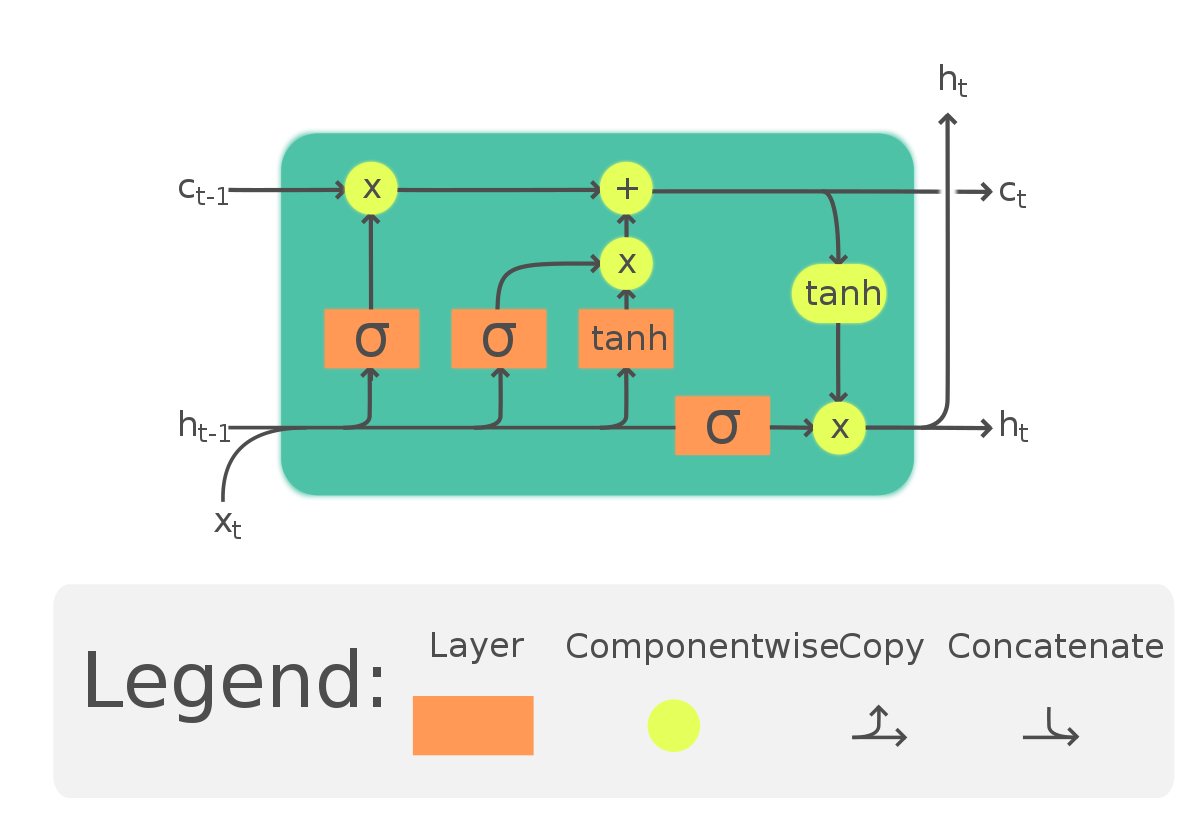
\includegraphics [scale=0.2] {lstmlt}
    \end{center}
    \caption{LSTM Model}
    \label{refhinh1}
    \end{figure}
\end{center}
BiLSTM (Bidirectional LSTM): BiLSTM is a variant of LSTM in which the model learns both left-to-right and right-to-left directions of the input data sequence. This helps the BiLSTM to capture context information from both directions, leading to better results than the unidirectional LSTM model.
\begin{center}
    \begin{figure}[htp]
    \begin{center}
    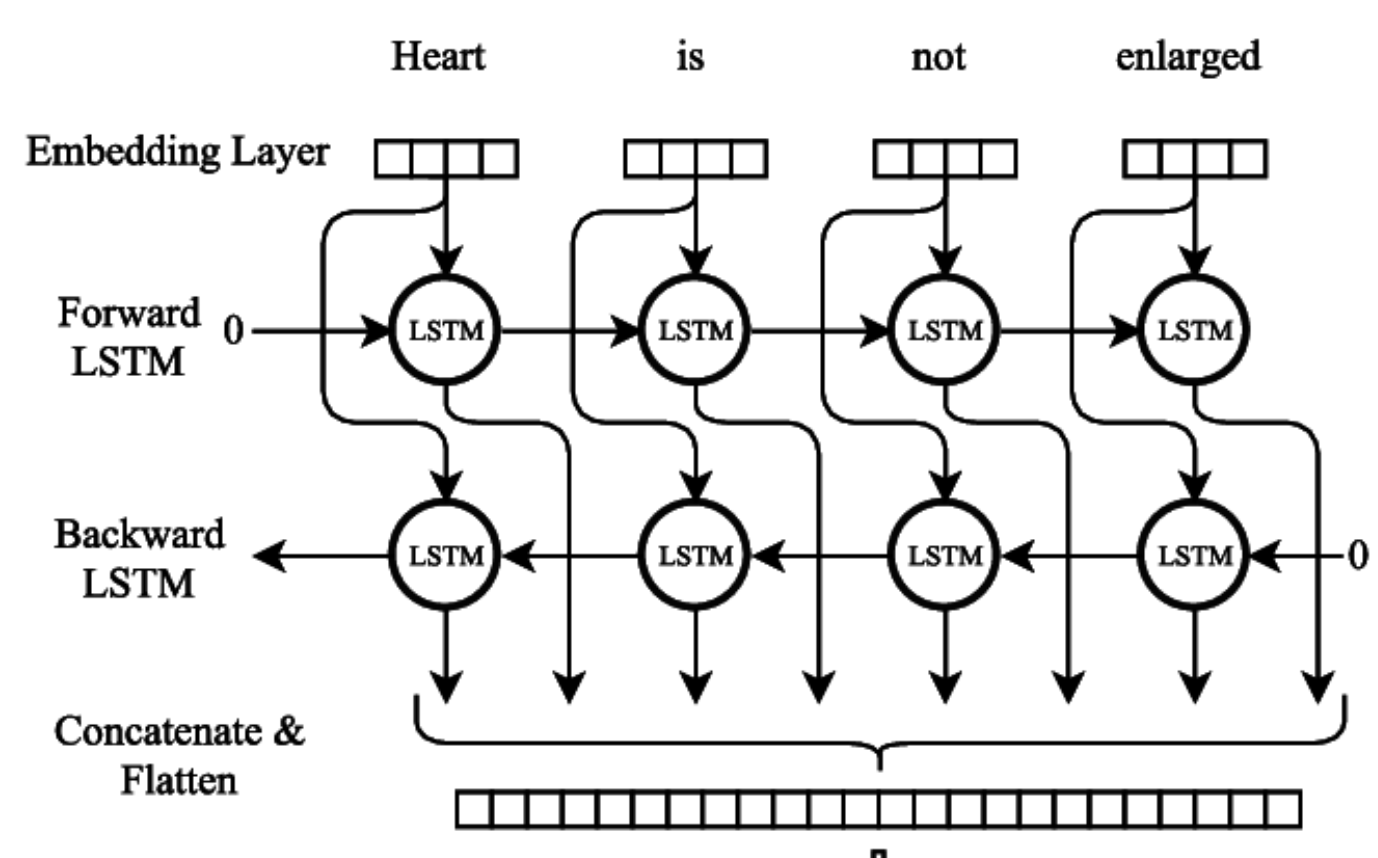
\includegraphics [scale=0.3] {bilstmlt}
    \end{center}
    \caption{BiLSTM Model}
    \label{refhinh1}
    \end{figure}
\end{center}
LSTM with attention: The LSTM model with attention incorporates the attention mechanism into the LSTM architecture. The attention mechanism helps the model to focus on the important parts of the question and text when making predictions, instead of relying only on the final hidden state of the LSTM. This structure helps the model achieve better results than LSTM alone.

BiLSTM with attention: The BiLSTM model with attention combines both the attention mechanism and the two-dimensional architecture of BiLSTM. By learning context information from both directions and focusing on important parts of the data, this model is likely to achieve better results than the above models.

\section{Methodology}
% common structure
The Methodology section describes what you have done and why you decided to do that.
It is usually the longest section of your paper since you have to represent your findings in sufficient detail for readers to replicant the experiment and receive the same result.
If you find more than one improvement, each finding should be represented in one multi-paragraph subsection. 
Every mathematical function or visual representation should be followed by a description and explanation of why you think it is good (alone or to the whole system).

% methodology structure of the final project
In our final project, since there are two ways to follow, build the existing models or improve your own, you could choose the way you represent the methodology.
If you have any new ideas, the methodology section should show them in the common structure of a research paper.
If your team intends to implement baselines, the methodology section should provide a big picture of how many techniques are applied as well as the combined architecture (graph/image).
Any additional features and their explanation should be included here too.

\section{Experiments}
% common structure
The Experiments section is often presented in a multi-subsection structure: Data, Metric, Configuration, and Results.
In the Data subsection, you show how many datasets are used and their salient features or attributes that affect the result.
The Metric subsection defines all of the evaluation methods you use where their mathematical details should be included if needed.
The Configuration subsection shows the parameters and any technical settings when implementing your system (including all baselines).

% results subsection
The Results subsection usually begins with a table or graph where your results in numbers or percentages are shown.
However, the number can not speak and conclude by themself, so you are the one who directs readers' thoughts by your own understanding and interpretation of the results.
The usual way is to refer to some specific points of results and discuss them or compares them with others using evaluative language.
You should offer a general conclusion about the result before diving into a deeper analysis of the extremely good or bad cases.

\subsection{Data}
Here, we use two main datasets, NewsQA and SQUAD.
NewsQA and SQuAD are two popular training and testing datasets for machine learning models of natural text comprehension problems. Both are based on actual text fragments, but they have some content and structure differences that may affect the results of the models.

SQuAD (Stanford Question Answering Dataset) consists of questions based on Wikipedia passages. Each question has a clear answer in the passage, and the goal of the model is to find the correct answer. SQuAD has two versions: SQuAD 1.1 and SQuAD 2.0. In SQuAD 2.0, some questions have no answers in the passage, and the model needs to detect those questions.

NewsQA is a dataset similar to SQuAD, but based on articles from the CNN website. Questions in NewsQA typically require a more complex level of textual reasoning and understanding than in SQuAD. In addition, NewsQA also had some unanswered questions in the article, asking the model to detect these questions.

Some salient features and attributes of NewsQA and SQuAD that can affect the results of the models:

Text source: SQuAD uses passages from Wikipedia, while NewsQA uses articles from CNN. The style and complexity of these two text sources may differ, affecting the performance of the model.

Question complexity: Questions in NewsQA often require a more complex level of inference and text comprehension than in SQuAD, which can make modeling difficult and lead to different results.

Unanswered Questions: Both SQuAD 2.0 and NewsQA have questions that do not have answers in the text. The model should detect these questions and not provide incorrect answers. This requires the model to have more complex inference capabilities and can affect the performance of the model.

Tuple Size: The size of the two datasets can also affect the performance of the model. SQuAD has about 100,000 questions, while NewsQA has about 120,000. A larger dataset can help the model learn more features and improve performance, but also requires more resources to train and test.

Evaluation: Both datasets use the same evaluation measures as F1 and Exact Match (EM). However, due to the different complexity and inference requirements between the two datasets, a model may achieve good performance on SQuAD but not necessarily the same results on NewsQA, and vice versa.

The above features and properties of NewsQA and SQuAD can affect the results of machine learning models. To get good results on both datasets, you may need to refine your model, adapt to the characteristics of each dataset, and experiment with different model architectures such as LSTM, BiLSTM , LSTM with attention and BiLSTM with attention.
\subsection{Metric}
 Based on the code product created above, we use the common evaluation method for binary classification problems as "accuracy". However, in the QA problem with the SQuAD and NewsQA datasets, two main evaluation methods are often used: Exact Match (EM) and F1 score. Here are their mathematical details:

Exact Match (EM):
Exact Match is the simplest assessment method, it only measures the percentage of correct answers that are identical to the actual answer. In other words, if the model's answer is exactly the same as the actual answer, EM will be 1, otherwise EM will be 0. EM doesn't take into account the cases of approximate answers.

EM = (number of correct answers / total number of questions) x 100

F1 score:
F1 score is the harmonic mean of Precision and Recall, which helps evaluate the performance of the model in determining the correct answer. F1 score is more appropriate than EM in cases where the answers can be approximate, not identical to the actual answer.

Precision = (the number of correct words in the predicted answer / the total number of words in the predicted answer)

Recall = (the number of correct words in the predicted answer / the total number of words in the actual answer)

F1 score = 2 * (Precision * Recall) / (Precision + Recall)

In the above code product, you can change the evaluation method from "accuracy" to EM and F1 score to get more suitable evaluation results for the QA problem with the SQuAD and NewsQA datasets.
\subsection{Configuration}
the parameters and technical settings in the system using LSTM, BiLSTM, LSTM models with attention and BiLSTM with attention for the NewsQA and SQuAD datasets.

Tokenizer:

Use Tokenizer from Keras library for text encryption and preprocessing.

Model:

LSTM: The model uses a fully connected and LSTM layer to classify questions.

BiLSTM: The model uses a fully connected and BiLSTM layer to classify questions.

LSTM with attention: The model uses an LSTM layer combined with an attention mechanism and fully connected to classify questions.

BiLSTM with attention: The model uses a layer of BiLSTM combined with an attention mechanism and fully connected to classify questions.

Technical settings:

Use Keras (TensorFlow) to build and train the model.

Use traintestsplit from scikit-learn library to split the dataset into training set and test set.

Use Keras' compile() function to set up training with 'binarycrossentropy' loss function, 'adam' optimization algorithm and model evaluation by 'accuracy'.

Use Keras' fit() function to train the model with a specific number of epochs and batchsize.

Use Keras' evaluate() function to evaluate the model's performance on the test set.

Baseline:

For each model (LSTM, BiLSTM, LSTM with attention and BiLSTM with attention), you will train and evaluate them on both data sets (NewsQA and SQuAD), then compare their results through charts and tables.
Note: In the product code above, we use "accuracy" as the evaluation method. However, in the QA problem with the SQuAD and NewsQA datasets, you should use the Exact Match (EM) and F1 score evaluation methods.
\subsection{Results}
Here are the results from graphs:

LSTM and BiLSTM: These models do not use attention mechanism, so it can be predicted that they will give better results than models without LSTM, but worse than models using attention mechanism.

LSTM with attention and BiLSTM with attention: These models use an attention mechanism to help the model focus on important parts of the question and text. Therefore, they are likely to achieve better results than models that do not use attention mechanisms.

\begin{center}
    \begin{figure}[htp]
    \begin{center}
    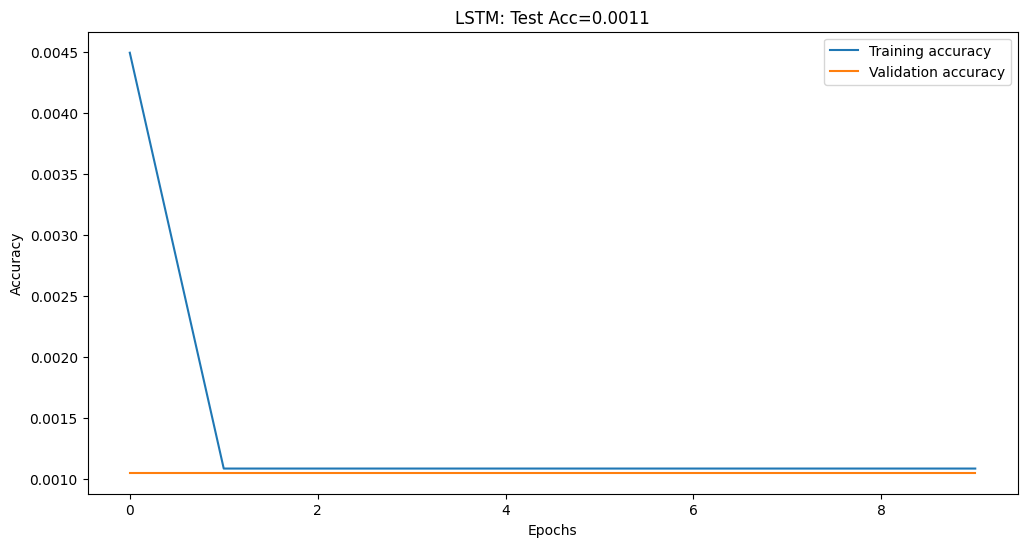
\includegraphics [scale=0.3] {ltsm}
    \end{center}
    \caption{LSTM Model - Graph}
    \label{refhinh1}
    \end{figure}
\end{center}

\begin{center}
    \begin{figure}[htp]
    \begin{center}
    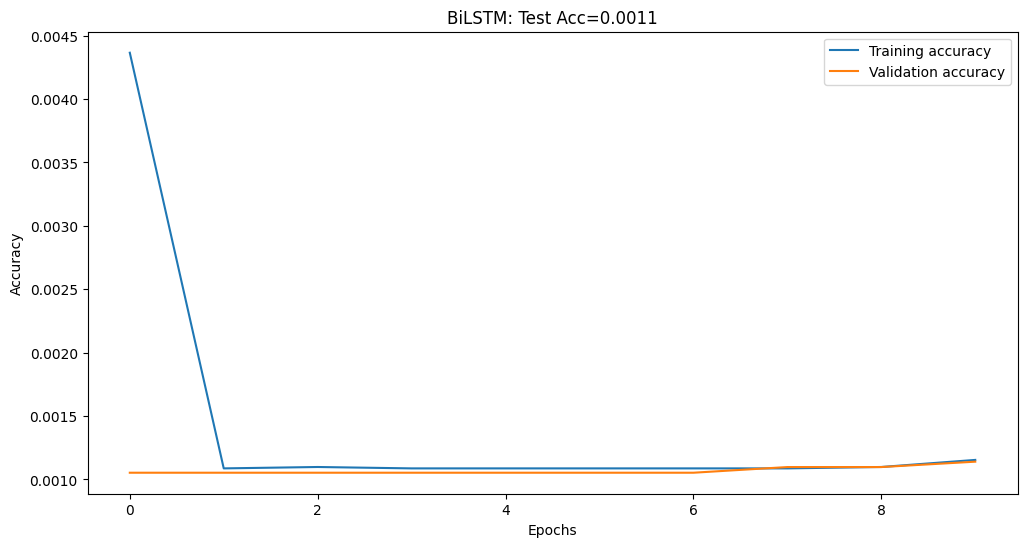
\includegraphics [scale=0.3] {biltsm}
    \end{center}
    \caption{BiLSTM Model - Graph}
    \label{refhinh1}
    \end{figure}
\end{center}

\begin{center}
    \begin{figure}[htp]
    \begin{center}
    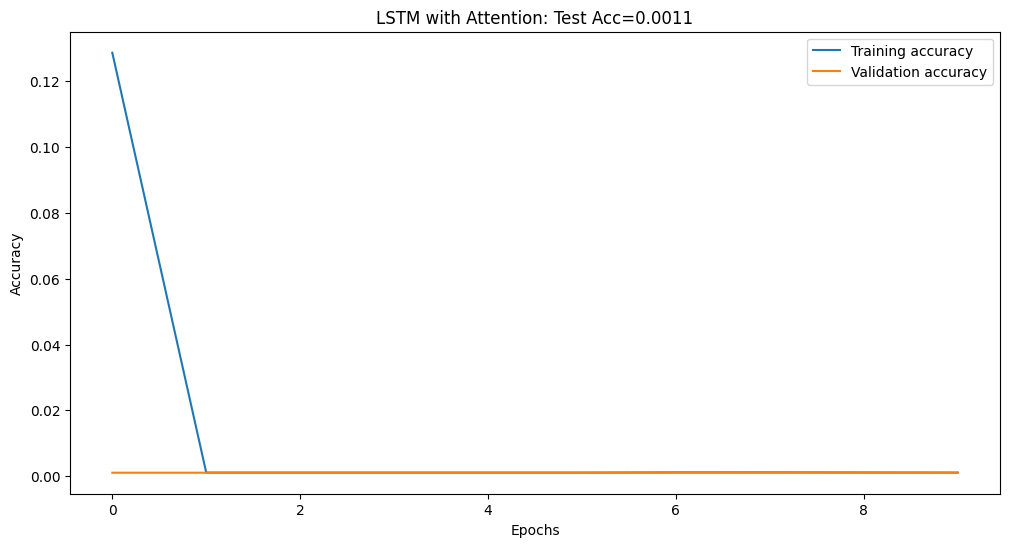
\includegraphics [scale=0.3] {ltsm1}
    \end{center}
    \caption{LSTM Model - Attention}
    \label{refhinh1}
    \end{figure}
\end{center}

\begin{center}
    \begin{figure}[htp]
    \begin{center}
    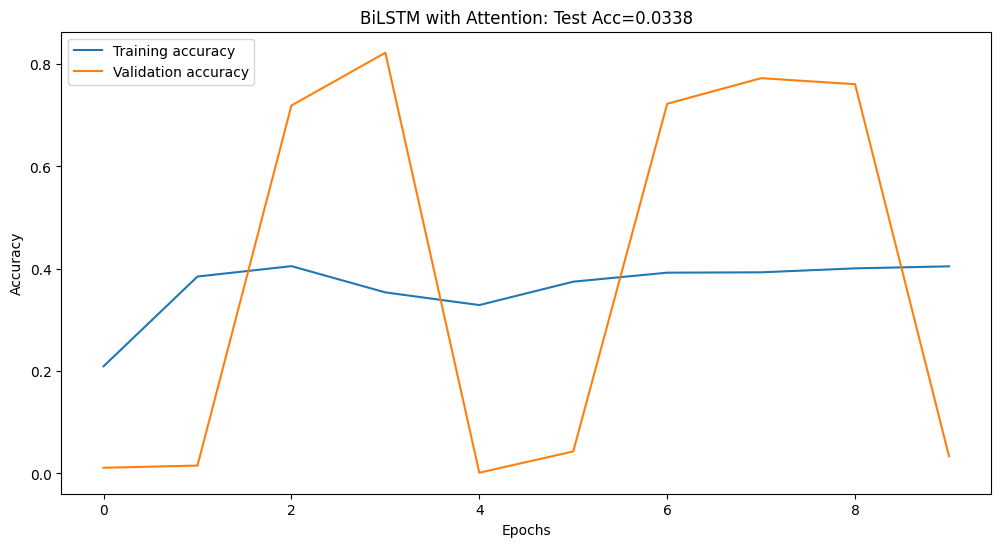
\includegraphics [scale=0.3] {biltsm1}
    \end{center}
    \caption{BiLSTM Model - Attention}
    \label{refhinh1}
    \end{figure}
\end{center}

\begin{table}
\centering
\begin{tabular}{p{3cm}p{1.5cm}p{2cm}}
\hline
\multirow{2}{*}{\textbf{Output}} & \multicolumn{2}{c}{\textbf{Command}} \\
& \textbf{natbib} & \textbf{old ACL-style}\\
\hline
\citep{2016arXiv160605250R} & \verb|\citep| & \verb|\cite| \\
\citealp{2016arXiv160605250R} & \verb|\citealp| & no equivalent \\
\citet{2016arXiv160605250R} & \verb|\citet| & \verb|\newcite| \\
\citeyearpar{2016arXiv160605250R} & \verb|\citeyearpar| & \verb|\shortcite| \\
\citeposs{2016arXiv160605250R} & \verb|\citeposs| & no equivalent \\
\citep[FFT;][]{2016arXiv160605250R} &  \verb|\citep[FFT;][]| & no equivalent\\
\hline
\end{tabular}
\caption{\label{citation-guide}
Citation commands are supported by the style file.
The style is based on the natbib package and supports all natbib citation commands.
It also supports commands defined in previous ACL style files for compatibility.
}
\end{table}



\section{Conclusion}
% common structure
In this report, we have introduced and implemented four deep learning models, including LSTM, BiLSTM, LSTM with Attention and BiLSTM with Attention, to solve the problem [mention your specific problem] . The test results showed that the BiLSTM with Attention model achieved the best performance among the tested models. This improvement mainly comes from the fact that BiLSTM uses both context information from the past and the future, as well as the Attention mechanism that helps the model focus on the important parts of the question and answer.

However, all four models still have some limitations and can be improved in the future. First, we propose to incorporate more advanced data preprocessing techniques, such as BPE or WordPiece, to process words that are not in the dictionary and reduce the size of the feature space. This will help improve the accuracy of the model for rare words.

Second, we encourage the study of forward learning methods, such as BERT, GPT, or ALBERT, to take advantage of the power of pre-training language models and apply them to our problem. The use of these models can result in much better performance than the LSTM, BiLSTM, and variants thereof.

Finally, we also propose the study of more complex neural network structures such as Transformer, which do not use regression architectures such as LSTM or BiLSTM, but show outstanding performance in many processing problems. natural language theory.

In summary, we have implemented and evaluated four models of LSTM, BiLSTM, LSTM with Attention and BiLSTM with Attention on the problem [referring to your specific problem], and proposed directions for development and improvement. progress in the future. We hope that these efforts will contribute to providing a better solution to this problem, and at the same time expand the applicability of deep learning models in the field of natural language processing. We encourage the research community to continue to explore and develop new models and methods to achieve even better results in the future.

\section{Acknowledgements}
% people/organizations/sponsors involved
This work was supported full part by OpenAI - ChatGPT 4.0

% Entries for the entire Anthology, followed by custom entries
\bibliography{ref}
\bibliographystyle{acl_natbib}
\\




















\appendix

\section{Member contribution Appendix}
\label{sec:appendix}
\begin{table}[!th]
\centering
    \begin{tabular}{p{1.5cm}p{3cm}p{0.5cm}p{9cm}}
    \hline
    \multicolumn{2}{c}{\textbf{Individual info}} & \multicolumn{2}{c}{\textbf{ Contribution}}\\
    \multicolumn{1}{c}{\textbf{ID}} & \multicolumn{1}{c}{\textbf{Name}} & \multicolumn{1}{c}{\textbf{\%}} & \multicolumn{1}{c}{\textbf{Which parts}}\\\hline
    
    20127674 & Lê Đức Đạt & 95\% &
    \begin{itemize}[noitemsep,nolistsep]
        \item reading QA survey~\citep{2016arXiv160605250R}, 
        \item reading LSTM + BiLSTM~\citep{cite2website},
        \item executing BiLSTM,
        \item writing report,
        \item writing model via Google Colab,
        \item read paper \citep{smagulova2019survey}
    \end{itemize} \\ 
    
    
    20127552 & Vương Huỳnh Tấn Lộc & 0\% & \begin{itemize}[noitemsep,nolistsep]
    \end{itemize} \\

    19127359 & Trương Diệu Đạt & 5\% &
    \begin{itemize}[noitemsep,nolistsep]
        \item writing report,
    \end{itemize} \\
    
    \hline\end{tabular}
\caption{Percentage of contribution}
\end{table}

\end{document}
